
% \begin{tikzpicture}[x=1cm,y=1cm,>=stealth]

% % ------------------------------------------------------------
% % Bounding box
% % ------------------------------------------------------------
% \path[use as bounding box] (0,2.15) rectangle (10.55,14.55);

% % ------------------------------------------------------------
% % Colours
% % ------------------------------------------------------------
% \definecolor{archline}{HTML}{2F425A}
% \definecolor{archtext}{HTML}{1E293B}

% \definecolor{aiborder}{HTML}{1261A8}
% \definecolor{aifill}{HTML}{DCEBFE}
% \definecolor{aiboxfill}{HTML}{BFDDFD}

% \definecolor{knowborder}{HTML}{26864A}
% \definecolor{knowfill}{HTML}{E1F4E5}
% \definecolor{knowboxfill}{HTML}{CDECD2}

% \definecolor{verborder}{HTML}{3F2C8C}
% \definecolor{verfill}{HTML}{EAE6FA}
% \definecolor{verboxfill}{HTML}{DCD3FC}

% \definecolor{execborder}{HTML}{B86F00}
% \definecolor{execfill}{HTML}{FEEDCD}
% \definecolor{execboxfill}{HTML}{FEE3A8}

% \definecolor{extborder}{HTML}{44556B}
% \definecolor{extfill}{HTML}{DCDDE2}

% % ============================================================
% % Outer system boundary
% % ============================================================

% \draw[
%     draw=extborder,
%     fill=white,
%     rounded corners=0.10cm,
%     line width=0.85pt
% ] (0.55,4.5) rectangle (10.00,12.75);


% % ============================================================
% % External entities
% % ============================================================

% % User
% \draw[
%     draw=extborder,
%     fill=extfill,
%     rounded corners=0.08cm,
%     line width=0.80pt
% ] (1.15,13.55) rectangle (3.05,14.25);

% \node[
%     font=\bfseries\fontsize{5.8}{6.3}\selectfont,
%     text=archtext
% ] at (2.10,13.90)
% {User};

% % Authoritative DeFi Sources
% \draw[
%     draw=extborder,
%     fill=extfill,
%     rounded corners=0.08cm,
%     line width=0.80pt
% ] (8.10,13.55) rectangle (10.10,14.38);

% \node[
%     font=\bfseries\fontsize{4.8}{5.3}\selectfont,
%     text=archtext,
%     align=center
% ] at (9.10,13.965)
% {Authoritative\\DeFi Sources};

% % Blockchain Network
% \draw[
%     draw=extborder,
%     fill=extfill,
%     rounded corners=0.08cm,
%     line width=0.80pt
% ] (6.95,3.47) rectangle (9.35,4.20);

% \node[
%     font=\bfseries\fontsize{5.4}{5.9}\selectfont,
%     text=archtext
% ] at (8.15,3.835)
% {Blockchain Network};

% % ============================================================
% % Group containers (2 x 2 arrangement)
% % ============================================================

% % AI / Intent
% \draw[
%     draw=aiborder,
%     fill=aifill,
%     rounded corners=0.10cm,
%     line width=0.85pt
% ] (1.00,9.10) rectangle (4.55,11.85);

% \node[
%     anchor=west,
%     font=\bfseries\fontsize{6.6}{7.1}\selectfont,
%     text=archline
% ] at (1.20,11.58)
% {AI / Intent};

% % Verification Knowledge
% \draw[
%     draw=knowborder,
%     fill=knowfill,
%     rounded corners=0.10cm,
%     line width=0.85pt
% ] (5.35,9.10) rectangle (9.55,11.85);

% \node[
%     anchor=west,
%     font=\bfseries\fontsize{6.3}{6.8}\selectfont,
%     text=archline
% ] at (5.55,11.58)
% {Verification Knowledge};

% % Relationship Verification
% \draw[
%     draw=verborder,
%     fill=verfill,
%     rounded corners=0.10cm,
%     line width=0.85pt
% ] (1.00,5.35) rectangle (4.55,8.10);

% \node[
%     anchor=west,
%     font=\bfseries\fontsize{6.1}{6.6}\selectfont,
%     text=archline
% ] at (1.20,7.83)
% {Relationship Verification};

% % Controlled Execution
% \draw[
%     draw=execborder,
%     fill=execfill,
%     rounded corners=0.10cm,
%     line width=0.85pt
% ] (5.35,5.35) rectangle (9.55,8.10);

% \node[
%     anchor=west,
%     font=\bfseries\fontsize{6.4}{6.9}\selectfont,
%     text=archline
% ] at (5.55,7.83)
% {Controlled Execution};

% % ============================================================
% % Internal component boxes
% % ============================================================

% % --- AI / Intent ---
% \draw[
%     draw=aiborder,
%     fill=aiboxfill,
%     rounded corners=0.07cm,
%     line width=0.80pt
% ] (1.35,10.32) rectangle (4.20,11.05);

% \node[
%     font=\bfseries\fontsize{5.1}{5.6}\selectfont,
%     text=archtext,
%     align=center
% ] at (2.775,10.685)
% {LLM-Based Intent Generation};

% \draw[
%     draw=aiborder,
%     fill=aiboxfill,
%     rounded corners=0.07cm,
%     line width=0.80pt
% ] (1.35,9.42) rectangle (4.20,10.05);

% \node[
%     font=\bfseries\fontsize{5.0}{5.5}\selectfont,
%     text=archtext,
%     align=center
% ] at (2.775,9.735)
% {Intent Validation};

% % --- Verification Knowledge ---
% \draw[
%     draw=knowborder,
%     fill=knowboxfill,
%     rounded corners=0.07cm,
%     line width=0.80pt
% ] (5.72,10.35) rectangle (9.18,11.08);

% \node[
%     font=\bfseries\fontsize{4.9}{5.4}\selectfont,
%     text=archtext,
%     align=center
% ] at (7.45,10.715)
% {Knowledge Acquisition \& Maintenance};

% \draw[
%     draw=knowborder,
%     fill=knowboxfill,
%     rounded corners=0.07cm,
%     line width=0.80pt
% ] (5.72,9.40) rectangle (9.18,10.12);

% \node[
%     font=\bfseries\fontsize{4.9}{5.4}\selectfont,
%     text=archtext,
%     align=center
% ] at (7.45,9.76)
% {Authoritative Property Graph};

% % --- Relationship Verification ---
% \draw[
%     draw=verborder,
%     fill=verboxfill,
%     rounded corners=0.07cm,
%     line width=0.80pt
% ] (1.45,6.38) rectangle (4.10,7.12);

% \node[
%     font=\bfseries\fontsize{5.0}{5.5}\selectfont,
%     text=archtext,
%     align=center
% ] at (2.775,6.75)
% {Relationship\\ Verification \& Decision};

% % --- Controlled Execution ---
% \draw[
%     draw=execborder,
%     fill=execboxfill,
%     rounded corners=0.07cm,
%     line width=0.80pt
% ] (5.78,6.58) rectangle (9.12,7.28);

% \node[
%     font=\bfseries\fontsize{4.9}{5.4}\selectfont,
%     text=archtext,
%     align=center
% ] at (7.45,6.93)
% {Verified-Result Validity Check};

% \draw[
%     draw=execborder,
%     fill=execboxfill,
%     rounded corners=0.07cm,
%     line width=0.80pt
% ] (5.78,5.68) rectangle (9.12,6.28);

% \node[
%     font=\bfseries\fontsize{4.8}{5.3}\selectfont,
%     text=archtext,
%     align=center
% ] at (7.45,5.98)
% {ERC-4337 Smart-Wallet Execution};

% % ============================================================
% % Subtle architectural connectors
% % ============================================================

% % User -- AI / Intent
% \draw[
%     draw=archline,
%     line width=0.75pt
% ] (2.10,13.55) -- (2.10,12.20) -- (2.35,12.20) -- (2.35,11.85);

% % AI / Intent -- Relationship Verification
% \draw[
%     draw=archline,
%     line width=0.75pt
% ] (2.775,9.10) -- (2.775,8.10);

% % Authoritative DeFi Sources -- Verification Knowledge
% \draw[
%     draw=archline,
%     line width=0.75pt
% ] (9.10,13.55) -- (9.10,12.30) -- (8.70,12.30) -- (8.70,11.85);

% % Verification Knowledge -- Relationship Verification
% \draw[
%     draw=archline,
%     line width=0.75pt
% ] (5.35,9.88) -- (4.85,9.88) -- (4.85,7.05) -- (4.55,7.05);

% % Relationship Verification -- Controlled Execution
% \draw[
%     draw=archline,
%     line width=0.75pt
% ] (4.55,6.72) -- (4.95,6.72) -- (4.95,6.72) -- (5.35,6.72);

% % Controlled Execution -- Blockchain Network
% \draw[
%     draw=archline,
%     line width=0.75pt
% ] (8.20,5.35) -- (8.20,4.50) -- (8.15,4.50) -- (8.15,4.20);

% % =========================================================
% % LEGEND 
% % =========================================================

% % Outer legend rectangle
% \draw[draw=extborder,rounded corners=0.06cm,line width=0.65pt]
%   (0.23,2.30) rectangle (10.32,3.01);

% % 1 AI
% \draw[draw=aiborder,fill=aifill,rounded corners=0.03cm,line width=0.60pt]
%   (0.38,2.49) rectangle (0.70,2.81);
% \node[anchor=west,text=archline] at (0.60,2.65)
%   {\scalebox{0.38}{AI / Intent Processing}};

% % 2 Verification
% \draw[draw=verborder,fill=verfill,rounded corners=0.03cm,line width=0.60pt]
%   (2.28,2.49) rectangle (2.60,2.81);
% \node[anchor=west,text=archline] at (2.55,2.65)
%   {\scalebox{0.38}{Relationship Verification}};

% % 3 Knowledge
% \draw[draw=knowborder,fill=knowfill,rounded corners=0.03cm,line width=0.60pt]
%   (4.35,2.49) rectangle (4.67,2.81);
% \node[anchor=west,text=archline] at (4.67,2.65)
%   {\scalebox{0.38}{Verification Knowledge}};

% % 4 Execution
% \draw[draw=execborder,fill=execfill,rounded corners=0.03cm,line width=0.60pt]
%   (6.42,2.49) rectangle (6.74,2.81);
% \node[anchor=west,text=archline] at (6.74,2.65)
%   {\scalebox{0.38}{Controlled Execution}};

% % 5 External
% \draw[draw=extborder,fill=extfill,rounded corners=0.03cm,line width=0.60pt]
%   (8.42,2.49) rectangle (8.74,2.81);
% \node[anchor=west,text=archline] at (8.70,2.65)
%   {\scalebox{0.38}{External Environment}};
% \end{tikzpicture}

% All information flows point from sender to receiver; see notation key.
\begingroup
\definecolor{archline}{HTML}{2F425A}
\definecolor{archtext}{HTML}{1E293B}
\definecolor{aiborder}{HTML}{1261A8}
\definecolor{aifill}{HTML}{DCEBFE}
\definecolor{knowborder}{HTML}{26864A}
\definecolor{knowfill}{HTML}{E1F4E5}
\definecolor{verborder}{HTML}{3F2C8C}
\definecolor{verfill}{HTML}{EAE6FA}
\definecolor{execborder}{HTML}{B86F00}
\definecolor{execfill}{HTML}{FEEDCD}
\definecolor{extborder}{HTML}{44556B}
\definecolor{extfill}{HTML}{DCDDE2}

\usetikzlibrary{arrows}
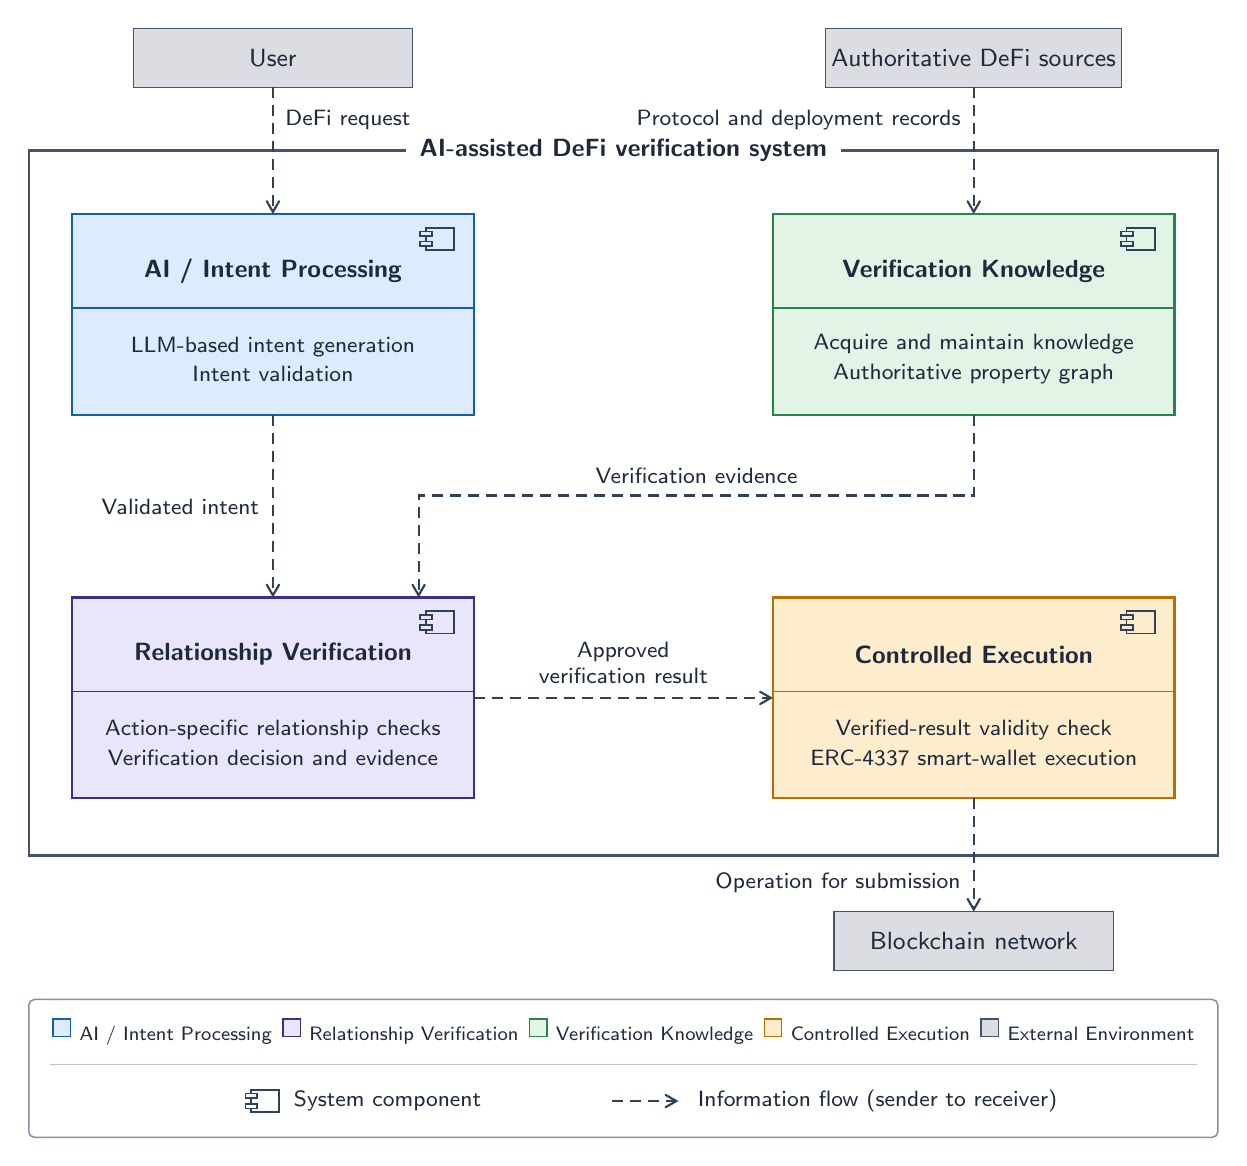
\begin{tikzpicture}[x=1cm,y=1cm,
 every node/.style={text=archtext,font=\sffamily\small,align=center},
 infoflow/.style={->,>=angle 60,draw=archline,dash pattern=on 4pt off 2.5pt,line width=.78pt},
 assoc/.style={draw=archline,line width=.78pt},
 labeltext/.style={font=\sffamily\footnotesize,inner sep=2pt},
 ext/.style={draw=extborder,fill=extfill,minimum width=3.55cm,
   minimum height=.75cm,inner sep=2pt,outer sep=0pt}]
% UML component glyph: a classifier rectangle with two protruding tabs.
\def\ArchGlyph#1#2#3{%
  \begin{scope}[shift={(#1,#2)},draw=archline,line width=.6pt]
    \draw[fill=#3] (-.18,-.14) rectangle (.18,.14);
    \draw[fill=#3] (-.25,.035) rectangle (-.10,.095);
    \draw[fill=#3] (-.25,-.095) rectangle (-.10,-.035);
  \end{scope}}
% The four equal component symbols have a header and a responsibility list.
% Parameters: name, x, y, outline, fill, title, responsibilities.
\def\ArchComponent#1#2#3#4#5#6#7{%
  \node[rectangle,draw=#4,fill=#5,line width=.85pt,
     minimum width=5.10cm,minimum height=2.55cm,inner sep=0pt,
     outer sep=0pt] (#1) at (#2,#3) {};
  \begin{scope}[shift={(#1.center)}]
    \ArchGlyph{2.12}{.96}{#5}
    \node[font=\sffamily\bfseries\small,inner sep=0pt] at (0,.55) {#6};
    \draw[draw=#4,line width=.55pt] (-2.55,.08) -- (2.55,.08);
    \node[inner sep=0pt,font=\sffamily\fontsize{8.1}{10.8}\selectfont] at (0,-.57) {#7};
  \end{scope}}
\draw[draw=extborder,line width=.85pt] (0,1.7) rectangle (15.1,10.65);
\node[anchor=center,fill=white,inner xsep=5pt,font=\sffamily\bfseries\small]
 at (7.55,10.65) {AI-assisted DeFi verification system};

\ArchComponent{ai}{3.1}{8.57}{aiborder}{aifill}{AI / Intent Processing}
  {LLM-based intent generation\\Intent validation}
\ArchComponent{knowledge}{12.0}{8.57}{knowborder}{knowfill}{Verification Knowledge}
  {Acquire and maintain knowledge\\Authoritative property graph}
\ArchComponent{verifier}{3.1}{3.70}{verborder}{verfill}{Relationship Verification}
  {Action-specific relationship checks\\Verification decision and evidence}
\ArchComponent{exec}{12.0}{3.70}{execborder}{execfill}{Controlled Execution}
  {Verified-result validity check\\ERC-4337 smart-wallet execution}

% External entities.
\node[ext] (user) at (3.1,11.83) {User};
\node[ext] (sources) at (12,11.83) {Authoritative DeFi sources};
\node[ext] (chain) at (12,.61) {Blockchain network};

% Labels identify the information conveyed, rather than the calling component.
\draw[infoflow] (user.south) -- (ai.north);
\node[labeltext,anchor=west] at (3.18,11.04) {DeFi request};
\draw[infoflow] (sources.south) -- (knowledge.north);
\node[labeltext,anchor=east] at (11.91,11.04) {Protocol and deployment records};

% The verifier has two independent inputs, with distinct arrow endpoints.
\draw[infoflow] (ai.south) -- (verifier.north);
\node[labeltext,anchor=east] at (3.00,6.13) {Validated intent};
\draw[infoflow] (knowledge.south) -- (12.0,6.27) -- (4.95,6.27)
  -- (4.95,4.975);
\node[labeltext,anchor=south] at (8.48,6.34) {Verification evidence};
\draw[infoflow] (verifier.east) -- (exec.west);
\node[labeltext,anchor=south] at (7.55,3.80) {Approved\\verification result};
\draw[infoflow] (exec.south) -- (chain.north);
\node[labeltext,anchor=east] at (11.91,1.35) {Operation for submission};

% One-row colour legend, with a separate notation key underneath.
\draw[draw=extborder!65,rounded corners=2pt,line width=.55pt]
  (0,-1.88) rectangle (15.10,-.13);
\def\ArchSwatch#1#2{%
  \tikz[baseline=-.48ex]{\draw[draw=#1,fill=#2,line width=.55pt]
       (0,0) rectangle (.22,.22);}\hspace{3pt}}
\node[inner sep=0pt,font=\sffamily\fontsize{7.4}{9.2}\selectfont]
 at (7.55,-.54) {\makebox[14.50cm][s]{%
  \ArchSwatch{aiborder}{aifill}AI / Intent Processing\hfill
  \ArchSwatch{verborder}{verfill}Relationship Verification\hfill
  \ArchSwatch{knowborder}{knowfill}Verification Knowledge\hfill
  \ArchSwatch{execborder}{execfill}Controlled Execution\hfill
  \ArchSwatch{extborder}{extfill}External Environment}};
\draw[draw=extborder!35,line width=.4pt] (.27,-.96) -- (14.83,-.96);
\ArchGlyph{3.0}{-1.42}{white}
\node[labeltext,anchor=west] at (3.29,-1.42) {System component};
\draw[infoflow] (7.41,-1.42) -- (8.25,-1.42);
\node[labeltext,anchor=west] at (8.42,-1.42)
  {Information flow (sender to receiver)};
\end{tikzpicture}
\endgroup